\documentclass[a4paper]{article}
\usepackage[utf8]{inputenc}
\usepackage[T1]{fontenc}
\usepackage{lmodern}
\renewcommand{\familydefault}{\sfdefault}
\usepackage[a4paper, margin=1.3cm, top=1.2cm, bottom=1.2cm]{geometry}
\setlength{\paperwidth}{210mm}
\setlength{\paperheight}{297mm}
\sloppy
\usepackage{enumitem}
\usepackage{xcolor}
\usepackage{graphicx}
\definecolor{darkblue}{rgb}{0,0,0.5}
\usepackage{hyperref}
\hypersetup{
    colorlinks=true,
    linkcolor=black,
    filecolor=black,
    urlcolor=darkblue,
    pdfstartview={FitH},
    pdfpagemode={UseNone}
}

\pagestyle{empty} % no page number

\setlength{\parindent}{0pt}

\newcommand{\sechead}[1]{
    \vspace{8pt}
    {\fontsize{13}{15}\bfseries #1} \par
    \vspace{3pt}
}

\newcommand{\entry}[2]{
    {\fontsize{10.5}{13}\fontseries{sb}\selectfont #1} \hfill {\fontsize{9}{11}\selectfont #2} \par
}

\newcommand{\desc}[1]{
    {\fontsize{9}{12.5}\selectfont #1}
}

\newcommand{\contactrow}[2]{
    {\fontsize{10}{14}\bfseries #1} {\fontsize{10}{14}\selectfont : #2} \par
}

\renewcommand{\labelitemi}{\fontsize{8}{10}\selectfont\textbullet}

\begin{document}

\begin{minipage}[c]{0.75\textwidth}
    {\fontsize{24}{28}\bfseries Yi\u{g}it Sarp Avc\i{}} \\[0.4em]
    {\fontsize{10}{12}\selectfont Istanbul, Turkey \quad \textbullet \quad +90 535 361 71 91 \quad \textbullet \quad yigitsarpavci@gmail.com} \\[0.3em]
    {\fontsize{10}{12}\selectfont LinkedIn: \href{https://www.linkedin.com/in/yigitsarpavci}{linkedin.com/in/yigitsarpavci} \quad \textbullet \quad GitHub: \href{https://github.com/yigitsarpavci}{github.com/yigitsarpavci}}
\end{minipage}%
\hfill
\begin{minipage}[c]{0.22\textwidth}
    \raggedleft
    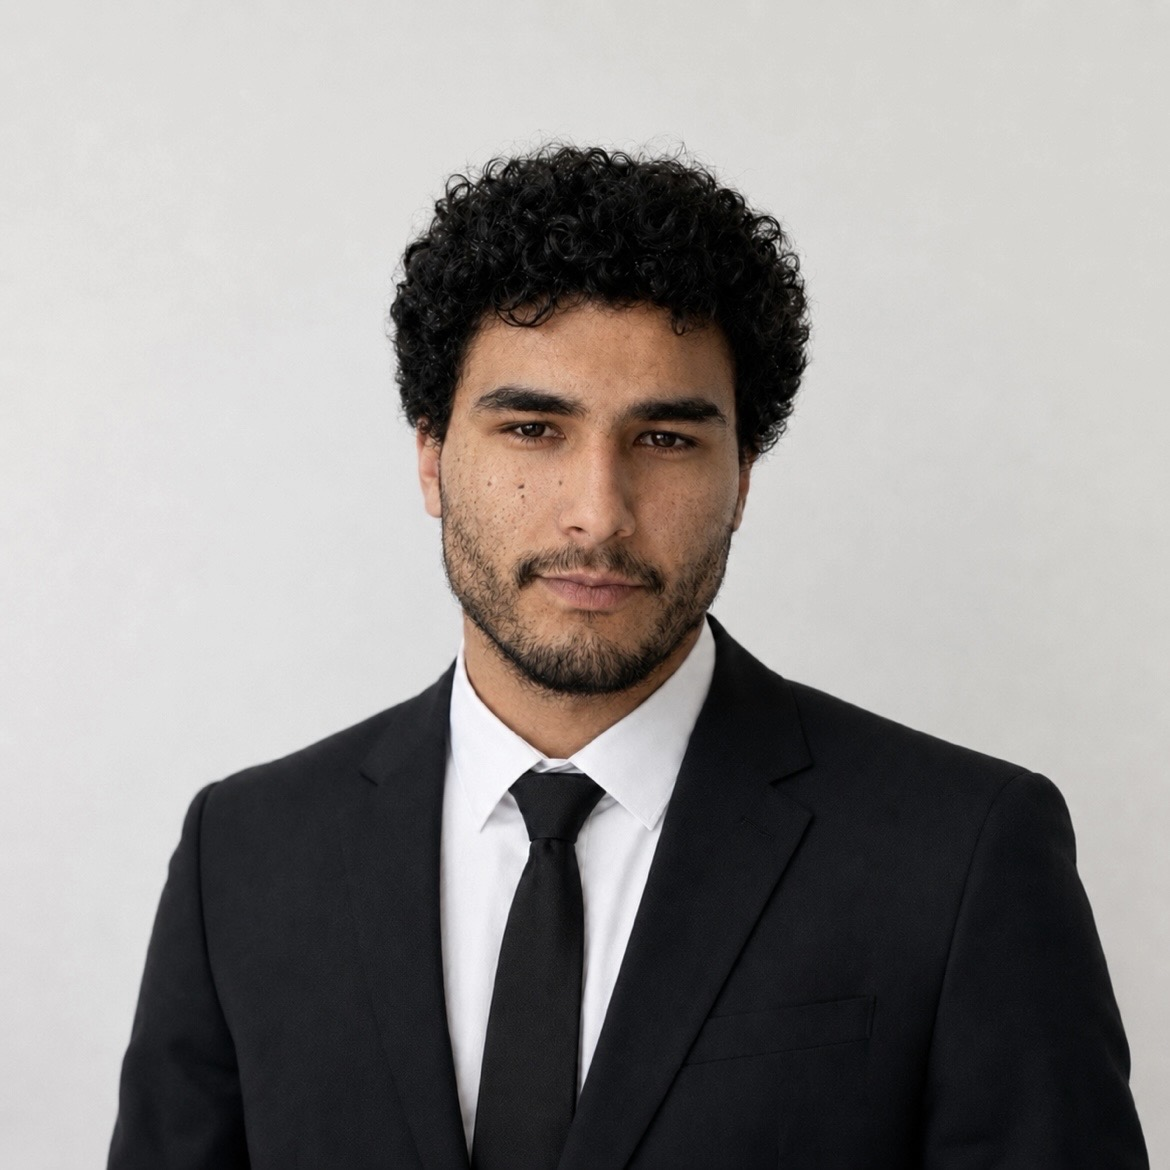
\includegraphics[width=2.5cm]{photocv.jpg}
\end{minipage}
\vspace{0.4em}

\sechead{Education}

\entry{Bo\u{g}azi\c{c}i University - B.Sc. in Computer Engineering}{09/2023 -- Present}
\begin{itemize}[leftmargin=1.1em, itemsep=0pt, parsep=0pt, topsep=2pt]
    \item \desc{Extracurriculars: Executive Board Member \& DJ at Radyo Bo\u{g}azi\c{c}i, Regional Organizational Team Member at ESTIEM; Student-Athlete (Sailing, Skiing \& Windsurfing), gave educational mentorship for high school students, participated in Work and Travel USA; Volunteer at Industrial Engineering Club.}
\end{itemize}
\vspace{4pt}

\entry{Kabata\c{s} Boys' High School}{09/2018 -- 06/2023}
\begin{itemize}[leftmargin=1.1em, itemsep=0pt, parsep=0pt, topsep=2pt]
    \item \desc{Graduated with a GPA of 3.78/4.00; Extracurriculars: Debate, Model United Nations, Entrepreneurship, and Coding Club; Volunteer: Kabata\c{s} Boys' High School CIP Club and TO\c{C}EV.}
\end{itemize}

\sechead{Experience}

\entry{Site Reliability Engineering Summer Intern at Akbank}{07/2026 -- Present}
\begin{itemize}[leftmargin=1.1em, itemsep=0pt, parsep=0pt, topsep=2pt]
   \item \desc{Joining the SRE team to contribute to the reliability, scalability, and performance of mission-critical banking systems. Excited to take on responsibilities involving infrastructure operations and systems engineering in a large-scale enterprise environment.}
\end{itemize}
\vspace{4pt}

\entry{Software Engineering Summer Intern at Smash Mate}{06/2026 -- 07/2026}
\begin{itemize}[leftmargin=1.1em, itemsep=0pt, parsep=0pt, topsep=2pt]
   \item \desc{Completed an intensive 1-month summer internship during the critical pre-launch phase, contributing to a complex microservices-oriented backend (Java, Quarkus) and a mobile frontend application (React Native). Developed core backend features, resolved high-priority issues, and authored comprehensive unit/integration tests to ensure zero-defect deployments. Played an active role in agile workflows, code reviews, and system optimizations, leading directly to the product's successful official launch.}
\end{itemize}
\vspace{2pt}




\sechead{Technical Projects \href{https://github.com/yigitsarpavci}{(@GitHub)}}

\entry{FinTech \& Trading Systems --- \textmd{Python, Next.js, FastAPI, PostgreSQL, Alembic, Pytest, WebSockets, Docker}}{}
\begin{itemize}[leftmargin=1.1em, itemsep=0pt, parsep=0pt, topsep=1pt]
   \item \desc{Developed \textbf{AlphaTrigger} (a real-time trading simulator featuring a Z-Score mean reversion strategy and volatility-adjusted position sizing) and the \textbf{FinTech Intelligence Platform} (featuring a live limit-order matching engine, portfolio risk analyzer, and AI-powered insights).}
\end{itemize}
\vspace{4pt}

\entry{Enterprise Dashboards \& Fullstack --- \textmd{Next.js 15+, TypeScript, Express, Prisma, TypeORM, Tailwind CSS, SWR}}{}
\begin{itemize}[leftmargin=1.1em, itemsep=0pt, parsep=0pt, topsep=1pt]
   \item \desc{Developed \textbf{Performo}, a real-time administrative dashboard with role-based access control, task management, and optimized database queries, alongside an \textbf{Enterprise FAQ System} featuring SWR-powered optimistic UI updates, Express backend, and robust API error boundaries.}
\end{itemize}
\vspace{4pt}

\entry{Systems \& CPU Scheduling --- \textmd{x86-64 Assembly, GNU Toolchain, Linux Syscalls, Process Scheduling, Multithreading (Pthreads), Memory Management}}{}
\begin{itemize}[leftmargin=1.1em, itemsep=0pt, parsep=0pt, topsep=1pt]
   \item \desc{Implemented \textbf{SchedSim}, a CPU scheduling simulator written in x86-64 GNU Assembly using direct Linux syscalls to execute FCFS, SJF, SRTF, Priority, and Round Robin scheduling algorithms.}
\end{itemize}
\vspace{4pt}

\entry{Interpreters \& Language Design --- \textmd{C, Python, Bash, Lexer Design, Functional Paradigms}}{}
\begin{itemize}[leftmargin=1.1em, itemsep=0pt, parsep=0pt, topsep=1pt]
   \item \desc{Built \textbf{Spireslayer} and \textbf{Aura}, including a C-based command interpreter with custom backtracking lexer/parser and a Python functional-language interpreter with closures, higher-order functions, and lexical/dynamic scoping.}
\end{itemize}
\vspace{4pt}

\entry{Algorithms \& Matching Engines --- \textmd{Java, Graph Theory, Heaps, Complexity Analysis}}{}
\begin{itemize}[leftmargin=1.1em, itemsep=0pt, parsep=0pt, topsep=1pt]
   \item \desc{Developed \textbf{MatrixNet} (a network graph analysis tool implementing Tarjan's SCC algorithm and articulation point detection) and \textbf{GigMatch-Pro} (a candidate matching engine using max-heap data structures for priority-based job allocation).}
\nolinebreak
\end{itemize}
\vspace{4pt}

\entry{Mobile Development, Game \& WebAssembly Engineering --- \textmd{React Native, Expo, C++, Qt6, WebAssembly, Java, TypeScript, Reanimated, Audio API, CI/CD}}{}
\begin{itemize}[leftmargin=1.1em, itemsep=0pt, parsep=0pt, topsep=1pt]
   \item \desc{Built \textbf{Smash Minesweeper} (a polished mobile app featuring a reducer-driven state engine, BFS flood-fill, and custom audio effects), \textbf{Qt 2048} (a C++/Qt6 clone cross-compiled to WebAssembly with undo history), and \textbf{Nightpass} (a terminal-based survival card game with a state-machine rule engine).}
\end{itemize}

\sechead{Skills}
\begin{itemize}[leftmargin=1.1em, itemsep=0pt, parsep=0pt, topsep=2pt]
   \item \desc{\textbf{Tools, AI \& Ecosystem:} Linux/Unix, Git/GitHub, AI-Assisted Development, ccache, Makefile, LaTeX, MS Office}
   \item \desc{\textbf{Languages:} Turkish (native), English (fluent), German (elementary)}
\end{itemize}


\end{document}
